% ---
% school: "college"
% level: "8eme"
% section: null
% chapter: "التناظر المركزي"
% source: "Axiomaths"
% title: "تقسيم قطعة أرض"
% country: "Tunisie"
% year: 2026
% professor: "Axiomaths"
% difficulty: "Difficile"
% points: null
% tags: ["symetrie-centrale", "aire", "parallelogramme", "probleme"]
% ---
% Exercice 15/19 de la série 8ème « التناظر المركزي » (statement + \axsol + solution). Compiler avec XeLaTeX + axiomath.sty (+ axiomaths-logo.png).
\documentclass[12pt,a4paper]{article}
\usepackage[level=8b,color=15803D]{axiomath}
\usetikzlibrary{arrows.meta}
\newcommand{\cm}{\,\mathrm{cm}}
\axsetup{title={التناظر المركزي}, corrige}

\begin{document}

\begin{corr}[title={تقسيم قطعة أرض}, stars=4, source={Axiomaths}]
قطعة أرض على شكل متوازي أضلاع $ABCD$ ، $AB=60\,\mathrm{m}$ وارتفاعها $30\,\mathrm{m}$ ، ومركزها $O$. يريد مالكها تقسيمها بممر مستقيم يمر من $O$ ويقطع $[AB]$ في $E$ حيث $AE=15\,\mathrm{m}$ وفي $[CD]$ في نقطة $F$.
\begin{center}
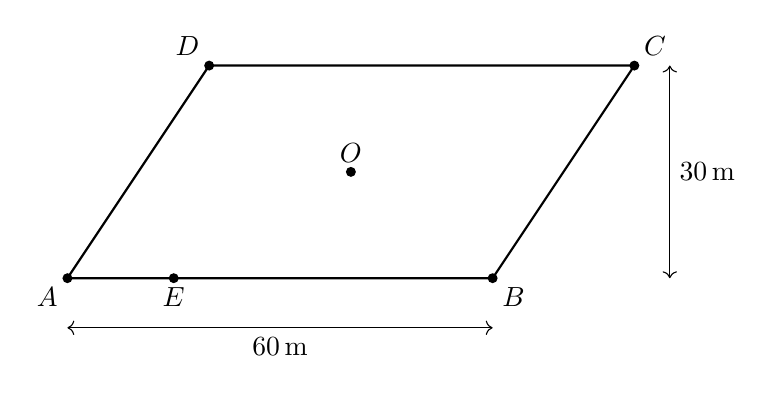
\begin{tikzpicture}[scale=0.9]
  \draw[thick] (0,0)--(6,0)--(8,3)--(2,3)--cycle;
  \fill (0,0) circle (2pt) node[below left] {$A$};
  \fill (6,0) circle (2pt) node[below right] {$B$};
  \fill (8,3) circle (2pt) node[above right] {$C$};
  \fill (2,3) circle (2pt) node[above left] {$D$};
  \fill (4,1.5) circle (2pt) node[above] {$O$};
  \fill (1.5,0) circle (2pt) node[below] {$E$};
  \draw[<->] (8.5,0)--(8.5,3) node[midway,right] {$30\,\mathrm{m}$};
  \draw[<->] (0,-0.7)--(6,-0.7) node[midway,below] {$60\,\mathrm{m}$};
\end{tikzpicture}
\end{center}
\begin{enumerate}
  \item بين أن $F$ مناظرة $E$ بالنسبة إلى $O$. احسب $CF$ و $DF$.
  \item احسب مساحة قطعة الأرض.
  \item بين أن الممر $[EF]$ يقسم القطعة إلى جزأين $AEFD$ و $EBCF$ متساويين في المساحة. ما مساحة كل منهما ؟
  \item تحقق من النتيجة بحساب مساحة شبه المنحرف $AEFD$.
  \item نغيّر موضع $E$ : $AE=x$ حيث $0<x<60$ (بالمتر). احسب مساحة $AEFD$ بدلالة $x$ ثم علّق.
\end{enumerate}
\axsol
\begin{enumerate}[itemsep=14pt]
  \item $S_O$ يحوّل $[AB]$ إلى $[CD]$ ($A\mapsto C$ و $B\mapsto D$) ، فمناظرة $E$ تنتمي إلى $[CD]$. وهي أيضا على المستقيم $(EO)$ لأن $O$ منتصف القطعة الواصلة بين $E$ ومناظرتها. والمستقيم $(EO)$ يقطع $(CD)$ في نقطة واحدة هي $F$. إذن $F=S_O(E)$.
  وبما أن $S_O$ يحفظ الأطوال ويحوّل $A$ إلى $C$ و $E$ إلى $F$ :
  \[CF=AE=15\,\mathrm{m}\]
  ومنه $DF=CD-CF=60-15=45\,\mathrm{m}$.
  \item مساحة متوازي الأضلاع = القاعدة $\times$ الارتفاع :
  \[\mathcal{A}(ABCD)=60\times30=1800\,\mathrm{m}^2\]
  \item $S_O$ يحوّل $A$ إلى $C$ و $E$ إلى $F$ و $F$ إلى $E$ و $D$ إلى $B$. إذن مناظر الرباعي $AEFD$ هو $CFEB$ أي $EBCF$. التناظر المركزي يحفظ المساحات ، إذن $\mathcal{A}(AEFD)=\mathcal{A}(EBCF)$. ومجموعهما $1800\,\mathrm{m}^2$ ، فلكل منهما :
  \[\dfrac{1800}{2}=900\,\mathrm{m}^2\]
  \item $AEFD$ شبه منحرف قاعدتاه $AE=15$ و $DF=45$ وارتفاعه $30$ :
  \[\mathcal{A}=\dfrac{(15+45)}{2}\times30=30\times30=900\,\mathrm{m}^2\ \checkmark\]
  \item $AE=x$ ، $CF=x$ ، $DF=60-x$. مساحة شبه المنحرف $AEFD$ :
  \[\dfrac{x+(60-x)}{2}\times30=\dfrac{60}{2}\times30=900\,\mathrm{m}^2\]
  لا تتوقف على $x$ : \ib{كل ممر يمر من $O$ يقسم القطعة إلى جزأين متساويين}. وهذا يتفق مع التناظر المركزي.
\end{enumerate}
\textbf{الفكرة :} برهانان : بالتناظر (دون حساب) وبالصيغة (بحساب). \quad \textbf{انتبه :} هذا غير صحيح لممر لا يمر من $O$.
\end{corr}

\end{document}
